\section*{Exercício 2}
Dados de leucemia (Feigl e Zelen, 1965): tempo de sobrevivência (semanas) de 33 pacientes, explicado por $\log(\text{WBC})$ e pelo fator AG (1 = positivo, 0 = negativo), supondo resposta gama.

\subsection*{Análise descritiva}

\begin{figure}[H]
\centering
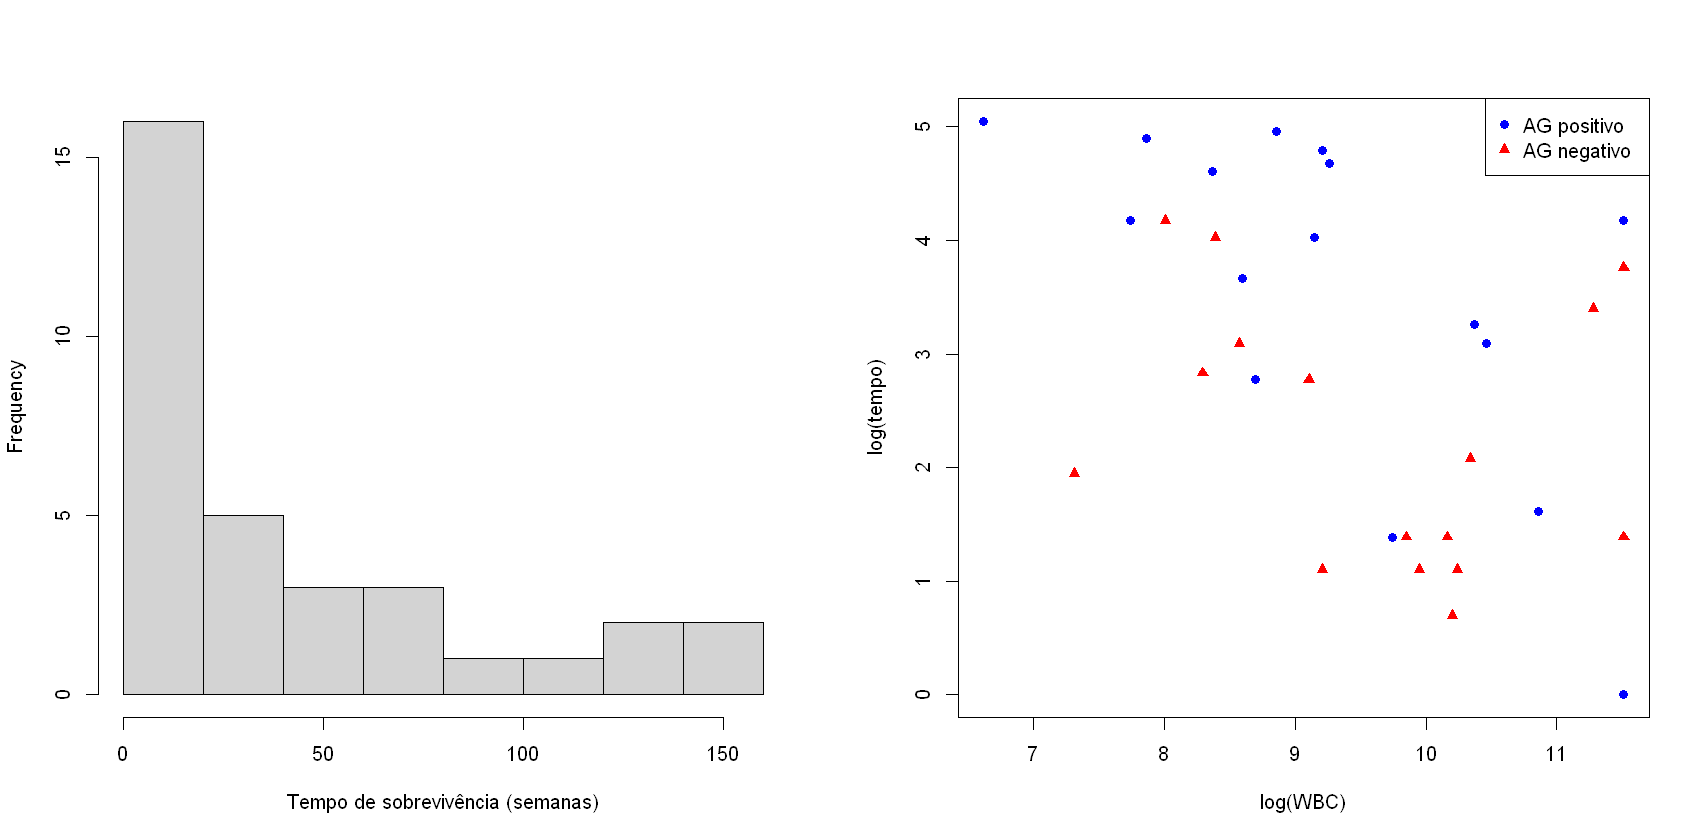
\includegraphics[width=0.6\textwidth]{ex2_descritiva.png}
\caption{Histograma do tempo (esquerda) e $\log(\text{tempo})$ contra $\log(\text{WBC})$ por grupo de AG (direita).}\label{fig:ex2desc}
\end{figure}

O tempo é bem assimétrico à direita (mediana 22, média 40,9, máximo 156), o que combina com a gama. Os pacientes AG positivo vivem bem mais em média (62,5 contra 17,9 semanas), e nos dois grupos o $\log(\text{tempo})$ cai quando o $\log(\text{WBC})$ aumenta (Figura~\ref{fig:ex2desc}).

\subsection*{Ajuste do modelo}

O modelo considerado foi $Y_i\sim\text{Gama}(\mu_i,\phi)$ com $\log\mu_i=\beta_0+\beta_1\log(\text{WBC}_i)+\beta_2\,\text{AG}_i$. Primeiro testamos a interação $\log(\text{WBC})\times\text{AG}$, que não é significativa ($F=1{,}58$; $p=0{,}219$). Por isso ficamos com o modelo aditivo (Tabela~\ref{tab:ex2coef}).

\begin{table}[H]
\centering\small
\caption{Estimativas do modelo gama aditivo (ligação log). IC de Wald para $\exp(\beta)$.}\label{tab:ex2coef}
\begin{tabular}{lrrrrl}
\toprule
Termo & Estimativa & EP & $p$ & $\exp(\hat\beta)$ & IC 95\% \\
\midrule
Intercepto & 5,815 & 1,349 & $<0{,}001$ & 335,43 & (23,85; 4716,58) \\
$\log(\text{WBC})$ & $-0{,}304$ & 0,138 & 0,035 & 0,738 & (0,563; 0,966) \\
AG & 1,018 & 0,364 & 0,009 & 2,767 & (1,355; 5,649) \\
\bottomrule
\end{tabular}
\end{table}

A dispersão do R é 1,088, ou seja, $\hat\phi\approx 0{,}92$ na parametrização do livro. Isso é bem perto de 1, então a distribuição está próxima de uma exponencial.

\subsection*{Diagnóstico}

\begin{figure}[H]
\centering
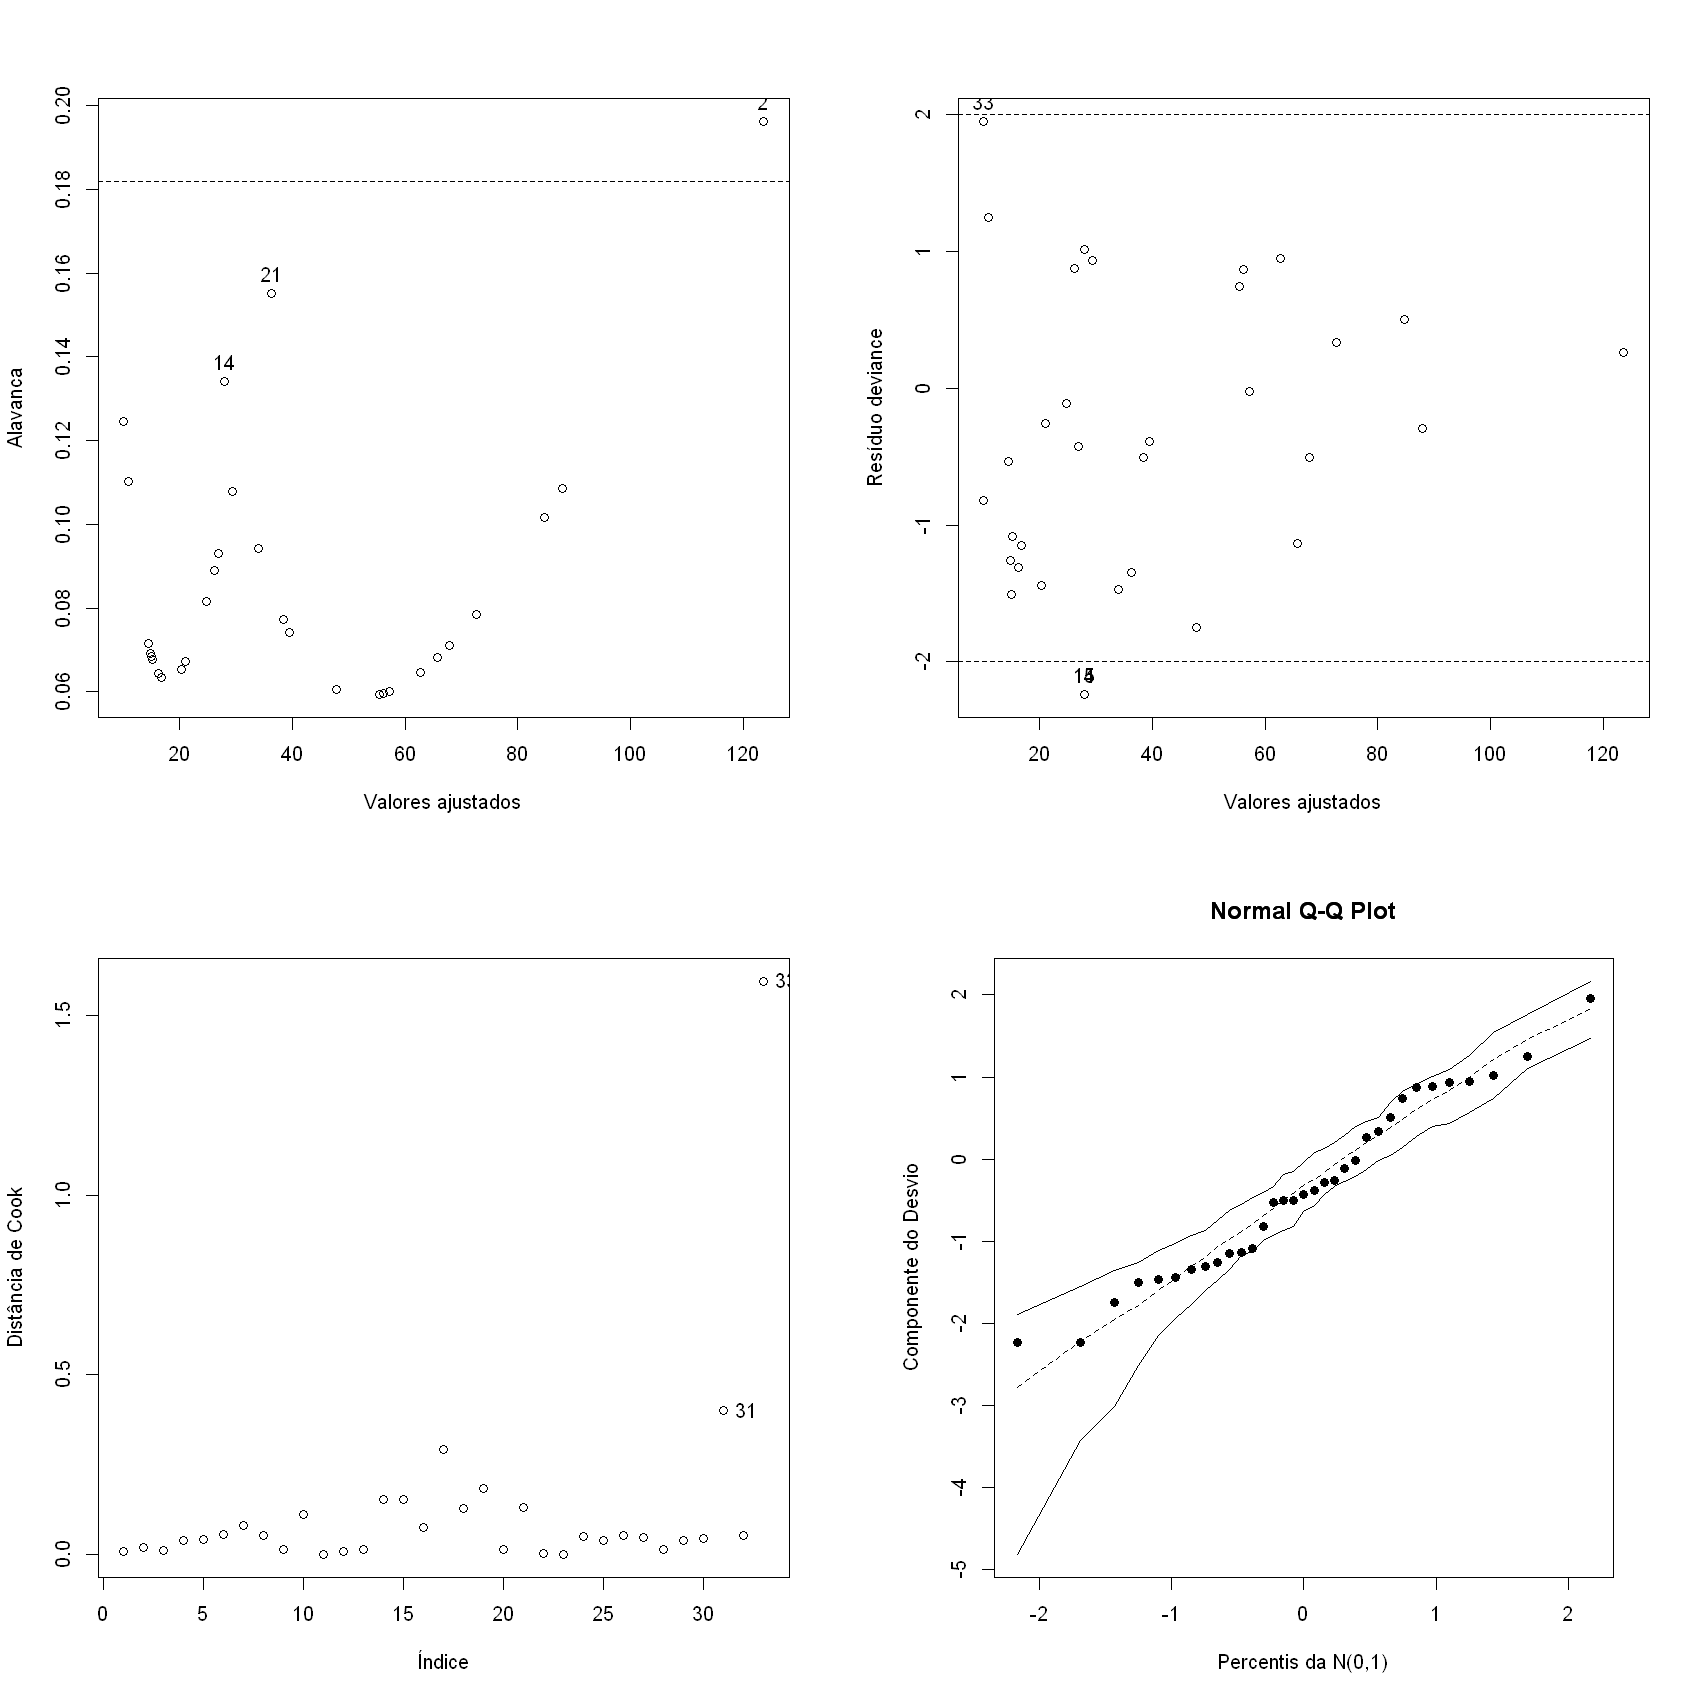
\includegraphics[width=\textwidth]{ex2_diag.png}
\caption{Alavanca, resíduo deviance padronizado, distância de Cook e envelope do modelo gama.}\label{fig:ex2diag}
\end{figure}

Resumindo a Figura~\ref{fig:ex2diag}:
\begin{itemize}[noitemsep]
\item \textbf{Alavanca:} só a obs.~2 (menor WBC, 750) passa um pouco da referência $2p/n=0{,}18$ ($h=0{,}196$), mas ela tem resíduo pequeno.
\item \textbf{Resíduo:} as obs.~14 e 15 (AG positivo, WBC = 100000, tempo = 1) são idênticas e ficam um pouco abaixo de $-2$ ($t_D=-2{,}24$). Elas viveram bem menos do que o esperado.
\item \textbf{Cook:} a obs.~33 (AG negativo, WBC = 100000, tempo = 43) se destaca bastante ($LD=1{,}59$). Ela sobreviveu muito mais do que o modelo prevê.
\item \textbf{Envelope:} todos os pontos ficam dentro das bandas, ou seja, não há evidência contra a gama.
\end{itemize}

\begin{table}[H]
\centering\small
\caption{Estimativas ($p$-valor) retirando as observações destacadas.}\label{tab:ex2sem}
\begin{tabular}{lcccc}
\toprule
Termo & Todas & Sem 33 & Sem 14 & Sem 14 e 15 \\
\midrule
$\log(\text{WBC})$ & $-0{,}304$ (0,035) & $-0{,}424$ (0,006) & $-0{,}268$ (0,062) & $-0{,}228$ (0,113) \\
AG & 1,018 (0,009) & 1,229 (0,003) & 1,107 (0,004) & 1,202 (0,002) \\
\bottomrule
\end{tabular}
\end{table}

Tirando a obs.~33 os efeitos ficam mais fortes, e tirando as obs.~14 e 15 o efeito de $\log(\text{WBC})$ perde significância (Tabela~\ref{tab:ex2sem}). Nenhum sinal muda e os tempos são plausíveis clinicamente, então mantemos todas as observações. Fica registrado que a significância de $\log(\text{WBC})$ depende desses dois pacientes.

\subsection*{GAMLSS: \texttt{plot}, \texttt{wp} e \texttt{term.plot}}

\begin{figure}[H]
\centering
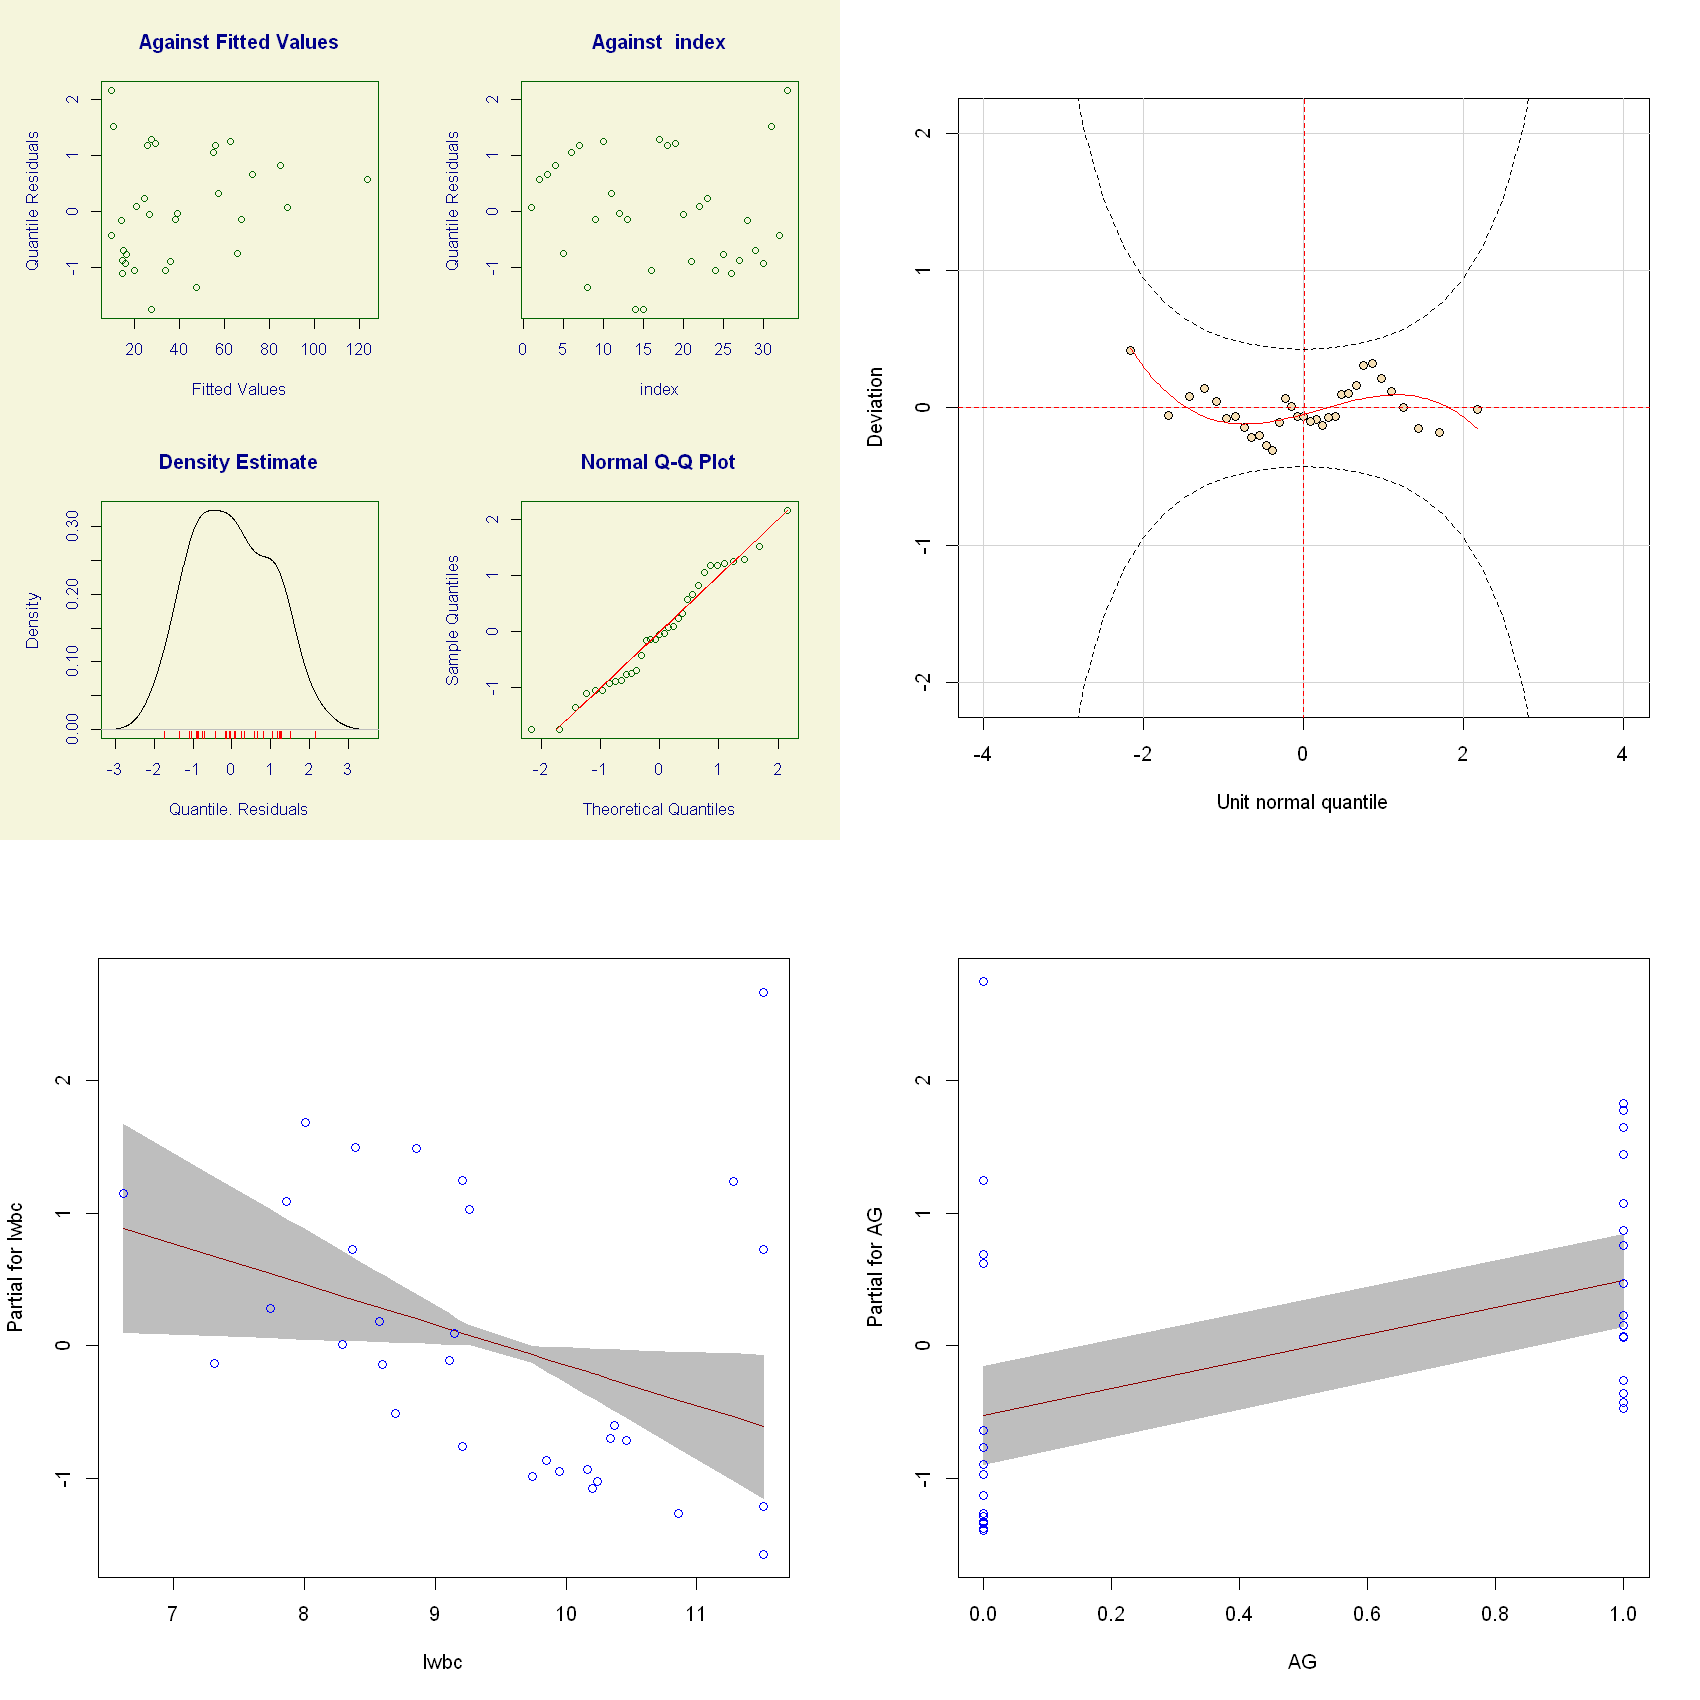
\includegraphics[width=\textwidth]{ex2_gamlss.png}
\caption{Ajuste no GAMLSS (família GA): \texttt{plot} dos resíduos quantílicos, \emph{worm plot} e \texttt{term.plot} de $\log(\text{WBC})$ e de AG.}\label{fig:ex2gamlss}
\end{figure}

As estimativas de $\mu$ no GAMLSS batem com as do \texttt{glm}, e $\hat\sigma=1{,}026$ (coeficiente de variação), de modo que $1/\hat\sigma^2=0{,}95$. Na Figura~\ref{fig:ex2gamlss}:
\begin{itemize}[noitemsep]
\item \textbf{\texttt{plot}:} os resíduos quantílicos não mostram tendência contra os ajustados nem contra o índice, e o QQ-plot fica perto da reta (média $-0{,}007$, variância 1,02, assimetria 0,16, Filliben 0,986). A curtose de 2,0 é um pouco baixa, mas com $n=33$ isso não preocupa.
\item \textbf{\texttt{wp}:} todos os pontos ficam dentro das curvas tracejadas e em torno do zero, sem forma marcada, ou seja, a distribuição está bem ajustada.
\item \textbf{\texttt{term.plot}:} o efeito parcial de $\log(\text{WBC})$ é uma reta decrescente (inclinação $\approx-0{,}30$), sem sinal de curvatura nos resíduos parciais. Para AG, a diferença entre os grupos é $\approx 1{,}02$ na escala log.
\end{itemize}

\subsection*{Interpretação}

O modelo ajustado é $\hat\mu=\exp\{5{,}815-0{,}304\log(\text{WBC})+1{,}018\,\text{AG}\}$, e os efeitos são multiplicativos no tempo médio:
\begin{itemize}[noitemsep]
\item \textbf{AG:} com o mesmo WBC, um paciente AG positivo vive em média $e^{1{,}018}\approx 2{,}8$ vezes mais que um AG negativo.
\item \textbf{WBC:} dobrar o WBC multiplica o tempo médio por $2^{-0{,}304}\approx 0{,}81$ (cerca de 19\% a menos), mantido o grupo AG.
\item \textbf{Intercepto:} não tem interpretação prática, porque corresponde a WBC = 1, muito fora da faixa observada.
\item \textbf{Dispersão:} o coeficiente de variação é $\approx 1$, ou seja, o desvio padrão do tempo é do tamanho da média. Mesmo pacientes com o mesmo perfil variam muito.
\end{itemize}
Em resumo: ser AG positivo está associado a maior sobrevivência, e mais células brancas no diagnóstico estão associadas a menor sobrevivência.
